\documentclass[a4paper, 12pt]{article}
\usepackage{cmap}
\usepackage{amssymb}
\usepackage{amsmath}
\usepackage{graphicx}
\usepackage{amsthm}
\usepackage{upgreek}
\setcounter{MaxMatrixCols}{11}
\usepackage{setspace}
\usepackage{color}
\usepackage{pgfplots}
\pgfplotsset{compat=1.9}
\usepackage[T2A]{fontenc}
\usepackage[utf8]{inputenc}
\usepackage[normalem]{ulem}
\usepackage{mathtext} % русские буквы в формулах
\usepackage[left=2cm,right=2cm, top=2cm,bottom=2cm,bindingoffset=0cm]{geometry}
\usepackage[english,russian]{babel}
\usepackage[unicode]{hyperref}
\newenvironment{Proof} % имя окружения
{\par\noindent{$\blacklozenge$}} % команды для \begin
{\hfill$\scriptstyle\boxtimes$}
\newcommand{\Rm}{\mathbb{R}}
\newcommand{\Cm}{\mathbb{C}}
\newcommand{\Z}{\mathbb{Z}}
\newcommand{\I}{\mathbb{I}}
\newcommand{\N}{\mathbb{N}}
\newcommand{\rank}{\operatorname{rank}}
\newcommand{\Ra}{\Rightarrow}
\newcommand{\ra}{\rightarrow}
\newcommand{\FI}{\Phi}
\newcommand{\Sp}{\text{Sp}}
\renewcommand{\leq}{\leqslant}
\renewcommand{\geq}{\geqslant}
\renewcommand{\alpha}{\upalpha}
\renewcommand{\beta}{\upbeta}
\renewcommand{\gamma}{\upgamma}
\renewcommand{\delta}{\updelta}
\renewcommand{\varphi}{\upvarphi}
\renewcommand{\phi}{\upvarphi}
\renewcommand{\tau}{\uptau}
\renewcommand{\lambda}{\uplambda}
\renewcommand{\psi}{\uppsi}
\renewcommand{\mu}{\upmu}
\renewcommand{\omega}{\upomega}
\renewcommand{\d}{\partial}
\renewcommand{\xi}{\upxi}
\renewcommand{\epsilon}{\upvarepsilon}
\newcommand{\intx}{\int\limits_{x_0}^x}
\newcommand\Norm[1]{\left\| #1 \right\|}
\newcommand{\sumk}{\sum\limits_{k=0}^\infty}
\newcommand{\sumi}{\sum\limits_{i=0}^\infty}
\newtheorem*{theorem}{Теорема}
\newtheorem*{cor}{Следствие}
\newtheorem*{lem}{Лемма}
\begin{document}
	\section*{Разностная аппроксимация дифференциального оператора}
	\subsubsection*{Условия}
	\begin{enumerate}
		\item Используя метод неопределенных коэффициентов, построить разностный оператор, аппроксимирующий дифференциальный оператор $Lu = u'(x)$ на шаблонах 
		\begin{enumerate}
			\item $\text{Ш}(x) = \{x, x+h\}$;
			\item $\text{Ш}(x) = \{x-h, x\}$;
			\item $\text{Ш}(x) = \{x-h, x, x+h\}$.
		\end{enumerate} 
		Определить порядок аппроксимации и главный член погрешности.
		(\hyperlink{t0}{Решение})
		\item Используя метод неопределенных коэффициентов, построить разностный оператор, аппроксимирующий $u''(x)$ на шаблоне $\text{Ш}(x) = \{x, x+h, x+2h\}$. Определить порядок аппроксимации и главный член погрешности. (\hyperlink{t1}{Решение})
		\item Используя метод неопределенных коэффициентов, построить разностный оператор, аппроксимирующий $u''(x)$ на шаблоне $\text{Ш}(x) = \{x-h, x, x+h\}$. Определить порядок аппроксимации и главный член погрешности. (\hyperlink{t2}{Решение})
		\item Используя метод неопределенных коэффициентов, построить разностный оператор, аппроксимирующий $u'(x)$ на нерегулярном шаблоне $\text{Ш}(x) = \{x-h_1, x, x+h_2\}$, $h_1 \ne h_2$. Определить порядок аппроксимации и главный член погрешности. (\hyperlink{t3}{Решение})
		\item Построить разностную аппроксимацию оператора $Lu$ методом неопределенных коэффициентов $$Lu = \dfrac{\d^2 u(x_1, x_2)}{\d x_1^2}.$$
		$$
		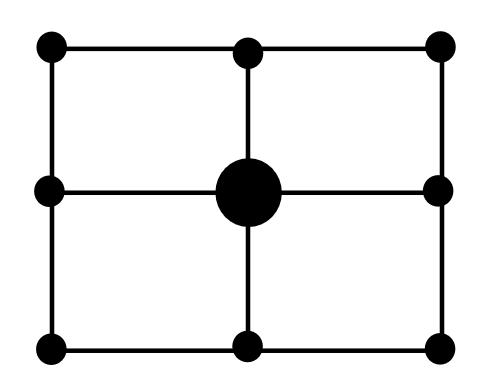
\includegraphics[scale=0.3]{images/img007}
		$$
		(\hyperlink{t4}{Решение})
	\end{enumerate}
	
	\newpage
	\subsubsection*{Решения}
	\begin{enumerate}
		\item \hypertarget{t0}{}
		\begin{enumerate}
			\item Итак, мы имеем дифференциальный оператор $$Lu = u'(x)$$ и шаблон $$\text{Ш}(x) = \{x, x+h\},$$ который можно изобразить как 
			$$
				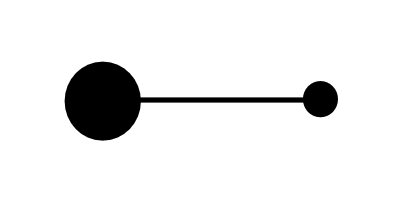
\includegraphics[scale=0.25]{images/img001}
			$$
			Разностную аппроксимацию будем искать в виде линейной комбинации значений функции $u(x)$ в точках шаблона, то есть $$L_h u(x) = a_0 u(x) + a_1 u(x+h).$$ Выпишем погрешность аппроксимации $\psi(x) = L_h u(x) - L u(x)$ в соответствии с нашими данными: $$\psi(x) = a_0 u(x) + a_1 u(x+h) - u'(x).$$
			Разложим правую часть этого уравнения в ряд Тейлора в окрестности точки $x$:
			\begin{equation*}
				\psi(x) = a_0 u(x) + a_1 \left(u(x) + h u'(x) + \dfrac{h^2}{2}u''(x) \right) + O(h^3) - u'(x) .
			\end{equation*}
			При необходимости можно записать и больше членов разложения. Теперь преобразуем выражение справа, вынеся общие множители, следующим образом
			\begin{equation*}
				\psi(x) = (a_0 + a_1)\cdot u(x) + (ha_1 -1 )\cdot  u'(x) + a_1\dfrac{h^2}{2}u''(x) +O(h^3).
			\end{equation*}
			Нас интересует возможность найти неизвестные коэффициенты $a_k$ такими, чтобы погрешность аппроксимации была минимальной. Для этого коэффициенты при $u(x)$, $u'(x)$ мы приравниваем к нулю и получаем следующую систему линейных уравнений для отыскания неизвестных коэффициентов 
			$$\begin{cases}
				a_0 + a_1= 0,\\
				ha_1  -1 = 0.
			\end{cases}$$
			Отсюда
			$$a_0 = -\dfrac{1}{h},\ a_1 = \dfrac{1}{h}.$$
			Таким образом, мы можем построить разностную аппроксимацию дифференциального оператора, подставив найденные коэффициенты в записанный ранее общий вид,
			$$L_h u(x) = \dfrac{u(x+h)  - u(x)}{h} = u_x.$$
			Построенная формула задает \textit{правую разностную производную}, которая обозначается символом $u_x$.\\\\ 
			Остается лишь определить порядок аппроксимации и главный член погрешности. Для этого найденные коэффициенты подставляем в нашу крайнюю запись для погрешности аппроксимации (учитываем, что первые два слагаемых обращаются в ноль при подстановке)
			$$
			\psi(x) = \dfrac{h}2 u''(x) + O(h^2) = O(h).
			$$
			То есть мы получаем аппроксимацию первого порядка, а главный член погрешности это $\dfrac{h}2 u''(x)$.
			Учитывая, что $$Lu = L_hu + \psi(x),$$
			можно записать выражение
			$$u'(x) = u_x + \dfrac{h}2 u''(x) + O(h^2) = \dfrac{u(x+h)  - u(x)}{h} + \dfrac{h}2 u''(x) + O(h^2),$$
			которое в последующих задачах будет использоваться.
			\item Итак, мы имеем дифференциальный оператор $$Lu = u'(x)$$ и шаблон $$\text{Ш}(x) = \{x-h, x\},$$ который можно изобразить как 
			$$
				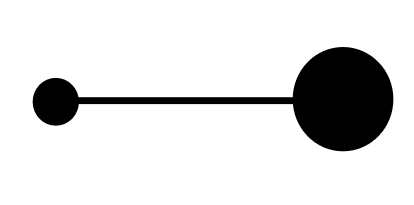
\includegraphics[scale=0.25]{images/img002}
			$$
			Разностную аппроксимацию будем искать в виде линейной комбинации значений функции $u(x)$ в точках шаблона, то есть $$L_h u(x) = a_0 u(x-h) + a_1 u(x).$$ Выпишем погрешность аппроксимации $\psi(x) = L_h u(x) - L u(x)$ в соответствии с нашими данными: $$\psi(x) = a_0 u(x-h) + a_1 u(x) - u'(x).$$
			Разложим правую часть этого уравнения в ряд Тейлора в окрестности точки $x$:
			\begin{equation*}
				\psi(x) = a_0 \left(u(x) - h u'(x) + \dfrac{h^2}{2}u''(x) \right) + a_1 u(x) + O(h^3) - u'(x) .
			\end{equation*}
			При необходимости можно записать и больше членов разложения. Теперь преобразуем выражение справа, вынеся общие множители, следующим образом
			\begin{equation*}
				\psi(x) = (a_0 + a_1)\cdot u(x) + (-ha_1 -1 )\cdot  u'(x) + a_1\dfrac{h^2}{2}u''(x) +O(h^3).
			\end{equation*}
			Нас интересует возможность найти неизвестные коэффициенты $a_k$ такими, чтобы погрешность аппроксимации была минимальной. Для этого коэффициенты при $u(x)$, $u'(x)$ мы приравниваем к нулю и получаем следующую систему линейных уравнений для отыскания неизвестных коэффициентов 
			$$\begin{cases}
				a_0 + a_1= 0,\\
				-ha_1  -1 = 0.
			\end{cases}$$
			Отсюда
			$$a_0 = -\dfrac{1}{h},\ a_1 = \dfrac{1}{h}.$$
			Таким образом, мы можем построить разностную аппроксимацию дифференциального оператора, подставив найденные коэффициенты в записанный ранее общий вид,
			$$L_h u(x) = \dfrac{u(x)  - u(x-h)}{h} = u_{\overline x}.$$
			Построенная формула задает \textit{левую разностную производную}, которая обозначается символом $u_{\overline x}$.\\\\ 
			Остается лишь определить порядок аппроксимации и главный член погрешности. Для этого найденные коэффициенты подставляем в нашу крайнюю запись для погрешности аппроксимации (учитываем, что первые два слагаемых обращаются в ноль при подстановке)
			$$
			\psi(x) = \dfrac{h}2 u''(x) + O(h^2) = O(h).
			$$
			То есть мы получаем аппроксимацию первого порядка, а главный член погрешности это $\dfrac{h}2 u''(x)$.
			Учитывая, что $$Lu = L_hu + \psi(x),$$
			можно записать выражение
			$$u'(x) = u_{\overline x} + \dfrac{h}2 u''(x) + O(h^2) = \dfrac{u(x)  - u(x-h)}{h} + \dfrac{h}2 u''(x) + O(h^2),$$
			которое в последующих задачах будет использоваться.
			\item Итак, мы имеем дифференциальный оператор $$Lu = u'(x)$$ и шаблон $$\text{Ш}(x) = \{x-h, x, x+h\},$$ который можно изобразить как 
			$$
				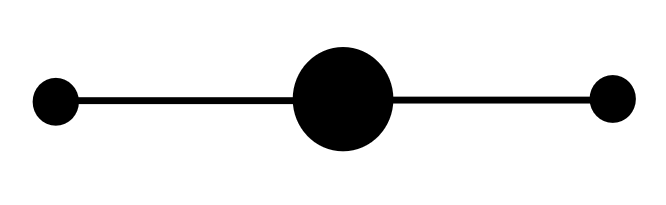
\includegraphics[scale=0.25]{images/img003}
			$$
			Разностную аппроксимацию будем искать в виде линейной комбинации значений функции $u(x)$ в точках шаблона, то есть $$L_h u(x) = a_0 u(x-h) + a_1 u(x) + a_2 u(x+h).$$ Выпишем погрешность аппроксимации $\psi(x) = L_h u(x) - L u(x)$ в соответствии с нашими данными: $$\psi(x) = a_0 u(x-h) + a_1 u(x) + a_2 u(x+h) - u'(x).$$
			Разложим правую часть этого уравнения в ряд Тейлора в окрестности точки $x$:
			\begin{multline*}
				\psi(x) = a_0 \left(u(x) - h u'(x) + \dfrac{h^2}{2}u''(x) - \dfrac{h^3}{6}u'''(x)  \right) + a_1 u(x) +\\+ a_2\left(u(x) + h u'(x) + \dfrac{h^2}{2}u''(x) + \dfrac{h^3}{6}u'''(x)  \right) + O(h^4) - u'(x) .
			\end{multline*}
			При необходимости можно записать и больше членов разложения. Теперь преобразуем выражение справа, вынеся общие множители, следующим образом
			\begin{multline*}
				\psi(x) = (a_0 + a_1+a_2)\cdot u(x) + (-ha_0 +ha_2 -1 )\cdot  u'(x) +\\+ \left(a_0\dfrac{h^2}{2} + a_2\dfrac{h^2}{2}\right)u''(x)+\left(-a_0\dfrac{h^3}{6} + a_2\dfrac{h^3}{6}\right)u'''(x) +O(h^3).
			\end{multline*}
			Нас интересует возможность найти неизвестные коэффициенты $a_k$ такими, чтобы погрешность аппроксимации была минимальной. Для этого коэффициенты при $u(x)$, $u'(x)$, $u''(x)$ мы приравниваем к нулю и получаем следующую систему линейных уравнений для отыскания неизвестных коэффициентов 
			$$\begin{cases}
				a_0 + a_1+a_2= 0,\\
				-a_0  +a_2 - \dfrac1h= 0,\\
				a_0 + a_2 = 0.
			\end{cases}$$
			Отсюда
			$$a_0 = -\dfrac{1}{2h},\ a_1 = 0, a_2 = \dfrac{1}{2h}$$
			Таким образом, мы можем построить разностную аппроксимацию дифференциального оператора, подставив найденные коэффициенты в записанный ранее общий вид,
			$$L_h u(x) = \dfrac{u(x+h)  - u(x-h)}{2h} = u_{\overset{\circ}{ x}}.$$
			Построенная формула задает \textit{центральную разностную производную}, которая обозначается символом $u_{\overset{\circ}{ x}}$.\\\\ 
			Остается лишь определить порядок аппроксимации и главный член погрешности. Для этого найденные коэффициенты подставляем в нашу крайнюю запись для погрешности аппроксимации (учитываем, что первые два слагаемых обращаются в ноль при подстановке)
			$$
			\psi(x) = \dfrac{h^2}6 u'''(x) + O(h^4) = O(h^2).
			$$
			То есть мы получаем аппроксимацию второго порядка, а главный член погрешности это $\dfrac{h^2}6 u'''(x)$.
			Учитывая, что $$Lu = L_hu + \psi(x),$$
			можно записать выражение
			$$u'(x) = u_{\overset{\circ}{ x}} + \dfrac{h^2}6 u'''(x) + O(h^4),$$
			которое в последующих задачах будет использоваться.
		\end{enumerate}
		\newpage
		\item \hypertarget{t1}{}
		Итак, мы имеем дифференциальный оператор $$Lu(x) = u''(x),$$ и шаблон $$\text{Ш}(x) = \{x, x+h, x+2h\}.$$ Разностную аппроксимацию будем искать в виде линейной комбинации значений функции $u$ в точках шаблона, то есть $$L_h u(x) = a_0 u(x) + a_1 u(x+h) + a_2 u(x+2h).$$ Выпишем погрешность аппроксимации $\psi(x) = L_h u(x) - L u(x)$ в соответствии с нашими данными: $$\psi(x) = a_0 u(x) + a_1 u(x+h) + a_2 u(x+2h) - u''(x).$$
		Разложим правую часть этого уравнения в ряд Тейлора в окрестности точки $x$:
		\begin{multline*}
			\psi(x) = a_0 u(x) + a_1 \left(u(x) + h u'(x) + \dfrac{h^2}{2}u''(x) + \dfrac{h^3}{6}u'''(x)\right) +\\+ a_2 \left(u(x) + 2h u'(x) + \dfrac{4h^2}{2}u''(x) + \dfrac{8h^3}{6}u'''(x)\right) + O(h^4) - u''(x) .
		\end{multline*}
		При необходимости можно записать и больше членов разложения. Теперь преобразуем выражение справа, вынеся общие множители, следующим образом
		\begin{multline*}
			\psi(x) = (a_0 + a_1 + a_2)\cdot u(x) + (ha_1 + 2ha_2)\cdot  u'(x) +\\+ \left(\dfrac{h^2}{2}a_1 + \dfrac{4h^2}{2}a_2 - 1\right)\cdot u''(x) + \left(\dfrac{h^3}{6}a_1 +\dfrac{8h^3}{6}a_2\right)\cdot u'''(x) +O(h^4).
		\end{multline*}
		Нас интересует возможность найти неизвестные коэффициенты $a_k$ такими, чтобы погрешность аппроксимации была минимальной. Для этого коэффициенты при $u(x)$, $u'(x)$, $u''(x)$ мы приравниваем к нулю и получаем следующую систему линейных уравнений для отыскания неизвестных коэффициентов 
		$$\begin{cases}
			a_0 + a_1 + a_2 = 0,\\
			ha_1  + 2ha_2  = 0,\\
			\dfrac{h^2}{2}a_1 + \dfrac{4h^2}{2}a_2 - 1 = 0.
		\end{cases}$$
		Домножим второе уравнение на $h$, а третье на 2 и получим
		$$\begin{cases}
			a_0 + a_1 + a_2 = 0,\\
			h^2 a_1+ 2 h^2 a_2= 0,\\
			h^2 a_1 + 4h^2a_2 = 2.
		\end{cases}$$
		Вычтем из третьего уравнения второе и получим 
		$$\begin{cases}
			a_0 + a_1 + a_2 = 0,\\
			h^2 a_1+ 2 h^2 a_2= 0,\\
			2h^2a_2 = 2.
		\end{cases}$$
		Отсюда $$a_2 = \dfrac{1}{h^2}.$$
		Тогда из второго уравнения $$a_1 = -\dfrac{2}{h^2},$$ а из первого уравнения $$a_0 = \dfrac{1}{h^2}.$$
		Таким образом, мы можем построить разностную аппроксимацию дифференциального оператора, подставив найденные коэффициенты в записанный ранее общий вид,
		$$L_h u(x) = \dfrac{u(x)  -2 u(x+h) +  u(x+2h)}{h^2}=u_{x x}.$$ 
		Остается лишь определить порядок аппроксимации и главный член погрешности. Для этого найденные коэффициенты подставляем в нашу крайнюю запись для погрешности аппроксимации (учитываем, что первые три слагаемых обращаются в ноль при подстановке)
		$$
		\psi(x) = \left(-\dfrac{h^3}{6}\cdot \dfrac{2}{h^2} +\dfrac{8h^3}{6} \cdot \dfrac{1}{h^2}\right)\cdot u'''(x) +O(h^4) = h u'''(x) + O(h^4) = O(h).
		$$
		То есть мы получаем аппроксимацию первого порядка, а главный член погрешности это $hu'''(x)$.
		
		\newpage
		\item 
		\hypertarget{t2}{}
		Итак, мы имеем дифференциальный оператор $$Lu(x) = u''(x),$$ и шаблон $$\text{Ш}(x) = \{x-h, x, x+h\}.$$ Разностную аппроксимацию будем искать в виде линейной комбинации значений функции $u$ в точках шаблона, то есть $$L_h u(x) = a_{-1} u(x-h) + a_0 u(x) + a_1 u(x+h).$$ Выпишем погрешность аппроксимации $\psi(x) = L_h u(x) - L u(x)$ в соответствии с нашими данными: $$\psi(x) = a_{-1} u(x-h) + a_0 u(x) + a_1 u(x+h) - u''(x).$$
		Разложим правую часть этого уравнения в ряд Тейлора в окрестности точки $x$:
		\begin{multline*}
			\psi(x) =  a_{-1} \left(u(x) - h u'(x) + \dfrac{h^2}{2}u''(x) - \dfrac{h^3}{6}u'''(x) + \dfrac{h^4}{24}u''''(x)\right) +a_0 u(x)\\+ a_1 \left(u(x) + h u'(x) + \dfrac{h^2}{2}u''(x) + \dfrac{h^3}{6}u'''(x) + \dfrac{h^4}{24}u''''(x)\right) + O(h^5) - u''(x) .
		\end{multline*}
		При необходимости можно записать и больше членов разложения. Теперь преобразуем выражение справа, вынеся общие множители, следующим образом
		\begin{multline*}
			\psi(x) = (a_{-1} + a_0 + a_1)\cdot u(x) + (-ha_{-1} + ha_1)\cdot  u'(x) + \left(\dfrac{h^2}{2}a_{-1} + \dfrac{h^2}{2}a_1 - 1\right)\cdot u''(x) +\\+ \left(-\dfrac{h^3}{6}a_{-1} +\dfrac{h^3}{6}a_1\right)\cdot u'''(x) + \left(\dfrac{h^4}{24}a_{-1} +\dfrac{h^4}{24}a_1\right)\cdot u''''(x) +O(h^5).
		\end{multline*}
		Нас интересует возможность найти неизвестные коэффициенты $a_k$ такими, чтобы погрешность аппроксимации была минимальной. Для этого коэффициенты при $u(x)$, $u'(x)$, $u''(x)$ мы приравниваем к нулю и получаем следующую систему линейных уравнений для отыскания неизвестных коэффициентов 
		$$\begin{cases}
			a_{-1} + a_0 + a_1= 0,\\
			-ha_{-1} + ha_1= 0,\\
			\dfrac{h^2}{2}a_{-1} + \dfrac{h^2}{2}a_1 - 1= 0.
		\end{cases}$$
		Домножим второе уравнение на $h$, а третье на 2 и получим
		$$\begin{cases}
			a_{-1} + a_0 + a_1= 0,\\
			-h^2 a_{-1}+ h^2 a_1= 0,\\
			h^2 a_{-1} + h^2a_1 = 2.
		\end{cases}$$
		Прибавим к третьему уравнению второе и получим
		$$\begin{cases}
			a_{-1} + a_0 + a_1= 0,\\
			-h^2 a_{-1}+ h^2 a_1= 0,\\
			2h^2a_1 = 2.
		\end{cases}$$
		Отсюда $$a_1 = \dfrac{1}{h^2}.$$
		Тогда из второго уравнения $$a_{-1} = \dfrac{1}{h^2},$$ а из первого уравнения $$a_0 = -\dfrac{2}{h^2}.$$
		Таким образом, мы можем построить разностную аппроксимацию дифференциального оператора, подставив найденные коэффициенты в записанный ранее общий вид,
		$$L_h u(x) = \dfrac{u(x-h)  -2 u(x) +  u(x+h)}{h^2} = u_{\overline x x}.$$ 
		Остается лишь определить порядок аппроксимации и главный член погрешности. Для этого найденные коэффициенты подставляем в нашу крайнюю запись для погрешности аппроксимации (учитываем, что первые три слагаемых обращаются в ноль при подстановке)
		\begin{multline*}
			\psi(x) = \left(-\dfrac{h^3}{6}\cdot \dfrac{1}{h^2} +\dfrac{h^3}{6} \cdot \dfrac{1}{h^2}\right)\cdot u'''(x) + \left(\dfrac{h^4}{24}\cdot \dfrac{1}{h^2} +\dfrac{h^4}{24} \cdot \dfrac{1}{h^2}\right)\cdot u''''(x)+\\ +O(h^5) = \dfrac{h^2}{12} u''''(x) + O(h^5) = O(h^2).
		\end{multline*}
		То есть мы получаем аппроксимацию второго порядка, а главный член погрешности это $\dfrac{h^2}{12} u''''(x)$.
	
	\newpage
	\item 
	\hypertarget{t3}{}
	Итак, мы имеем дифференциальный оператор $$Lu(x) = u'(x),$$ и нерегулярный шаблон (то есть с разным шагом) $$\text{Ш}(x) = \{x-h_1, x, x+h_2\},\ h_1 \ne h_2.$$ Разностную аппроксимацию будем искать в виде линейной комбинации значений функции $u$ в точках шаблона, то есть $$L_h u(x) = a_{-1} u(x-h_1) + a_0 u(x) + a_1 u(x+h_2).$$ Выпишем погрешность аппроксимации $\psi(x) = L_h u(x) - L u(x)$ в соответствии с нашими данными: $$\psi(x) = a_{-1} u(x-h_1) + a_0 u(x) + a_1 u(x+h_2) - u'(x).$$
	Разложим правую часть этого уравнения в ряд Тейлора в окрестности точки $x$:
	\begin{multline*}
		\psi(x) = a_0\left(u(x) - h_1u'(x) + \dfrac{h_1^2}{2}u''(x)-\dfrac{h_1^3}{6}u'''(x)\right) + a_1 u(x)\\+ a_2 \left(u(x) + h_2 u'(x) + \dfrac{h_2^2}{2}u''(x) +\dfrac{h_2^3}{6}u'''(x)\right) + O(h_1^4+h_2^4) - u'(x) .
	\end{multline*}
	При необходимости можно записать и больше членов разложения. Теперь преобразуем выражение справа, вынеся общие множители, следующим образом
	\begin{multline*}
		\psi(x) = (a_0 + a_1 + a_2)\cdot u(x) + (-h_1a_{0} + h_2a_2 - 1)\cdot  u'(x) +\\+ \left(\dfrac{h_1^2}{2}a_{0} + \dfrac{h_2^2}{2}a_2\right)\cdot u''(x) + \left(-\dfrac{h_1^3}{6}a_{0} + \dfrac{h_2^3}{6}a_2\right)u'''(x)+O(h_1^4+h_2^4).
	\end{multline*}
	Нас интересует возможность найти неизвестные коэффициенты $a_k$ такими, чтобы погрешность аппроксимации была минимальной. Для этого коэффициенты при $u(x)$, $u'(x)$, $u''(x)$ мы приравниваем к нулю и получаем следующую систему линейных уравнений для отыскания неизвестных коэффициентов 
	$$\begin{cases}
		a_0 + a_1 + a_2= 0,\\
		-h_1a_{0} + h_2a_2 - 1= 0,\\
		\dfrac{h_1^2}{2}a_{0} + \dfrac{h_2^2}{2}a_2 = 0.
	\end{cases}$$
	Домножим второе уравнение на $h_1$, а третье на 2 и получим
	$$\begin{cases}
		a_0 + a_1 + a_2= 0,\\
		-h_1^2 a_{0}+ h_1h_2 a_2= h_1,\\
		h_1^2 a_{0} + h_2^2a_2 = 0.
	\end{cases}$$
	Прибавим к третьему уравнению второе и получим
	$$\begin{cases}
		a_0 + a_1 + a_2= 0,\\
		-h_1^2 a_{0}+ h_1h_2 a_2= h_1,\\
		(h_1h_2 + h_2^2)a_2 = h_1.
	\end{cases}$$
	Отсюда $$a_2 = \dfrac{h_1}{h_2 (h_1+h_2)}.$$
	Тогда из второго уравнения $$a_{0} = \dfrac{h_2}{h_1 (h_1+h_2)},$$ а из первого уравнения $$a_1 = -\left(\dfrac{h_1^2+h_2^2}{h_1h_2}\right)\cdot \dfrac{1}{h_1+h_2}.$$
	Таким образом, мы можем построить разностную аппроксимацию дифференциального оператора, подставив найденные коэффициенты в записанный ранее общий вид,
	$$L_h u(x) = \dfrac{1}{h_1+h_2}\cdot\left(\dfrac{h_2^2 u(x-h_1) -(h_1^2+h_2^2)u(x) + h_1^2u(x+h_2)}{h_1h_2}\right).$$ 
	Остается лишь определить порядок аппроксимации и главный член погрешности. Для этого найденные коэффициенты подставляем в нашу крайнюю запись для погрешности аппроксимации (учитываем, что первые три слагаемых обращаются в ноль при подстановке)
	\begin{multline*}
		\psi(x) = \left(-\dfrac{h_1^3}{6}\cdot \dfrac{h_2}{h_1 (h_1+h_2)} +\dfrac{h_2^3}{6} \cdot \dfrac{h_1}{h_2 (h_1+h_2)}\right)\cdot u'''(x) +\\+O(h_1^4+h_2^4) = \dfrac{h_1h_2}{6(h_1+h_2)}(h_1-h_2)\cdot u''''(x) + O(h_1^4+h_2^4) = O(h_1^2+h_2^2).
	\end{multline*}
	То есть мы получаем аппроксимацию второго порядка, а главный член погрешности это $\dfrac{h_1h_2}{6(h_1+h_2)}(h_1-h_2)\cdot u''''(x)$.
	\newpage
	\item 
	\hypertarget{t4}{}
	Пусть у нас имеется равномерная сетка узлов.
	Разностную аппроксимацию будем искать в виде линейной комбинации значений функции $u$ в точках шаблона, то есть \begin{multline*}
		L_h u(x) = a_0 u(x_1, x_2) + a_1 u(x_1-h, x_2-h) + a_2 u(x_1-h, x_2) + a_3u(x_1-h, x_2 + h) + a_4 u(x_1, x_2-h) + \\+ a_5 u (x_1, x_2+h) + a_6 u(x_1 + h, x_2 - h) + a_7 u(x_1+h, x_2) + a_8u(x_1 + h, x_2+h).
	\end{multline*} Выпишем погрешность аппроксимации $\psi(x) = L_h u(x) - L u(x)$ в соответствии с нашими данными: 
	\begin{multline*}
		\psi(x) = a_0 u(x_1, x_2) + a_1 u(x_1-h, x_2-h) + a_2 u(x_1-h, x_2) + a_3u(x_1-h, x_2 + h) + a_4 u(x_1, x_2-h) + \\+ a_5 u (x_1, x_2+h) + a_6 u(x_1 + h, x_2 - h) + a_7 u(x_1+h, x_2) + a_8u(x_1 + h, x_2+h) - \dfrac{\d^2 u(x_1, x_2)}{\d x_1^2}.
	\end{multline*}
	Разложим правую часть этого уравнения в ряд Тейлора, используя формулу разложения функции двух переменных \begin{multline*}
		u(x,y) = u(x_0, y_0) + \dfrac{1}{1!}\left(\dfrac{\d }{\d x}(x-x_0) +\dfrac{\d }{\d y}(y-y_0)\right)^2u(x_0, y_0) +\\+  \dfrac{1}{2!}\left(\dfrac{\d }{\d x}(x-x_0) +\dfrac{\d }{\d y}(y-y_0)\right)^2u(x_0, y_0) + \ldots,
	\end{multline*} в окрестности точек $x_1, x_2$ по степеням $h$. Для упрощения записи, сразу же будем выносить общие множители за скобки, тогда
	\begin{multline*}
		\psi(x) = u\cdot (a_0 + a_1 + a_2 + a_3 + a_4 + a_5 + a_6 + a_7 + a_8) + \\ + h\dfrac{\d u}{\d x_1} (-a_1 -a_2 -a_3 + a_6 + a_7 + a_8) + h\dfrac{\d u}{\d x_2} (-a_1 +a_3 - a_4 + a_5 - a_6 + a_8) + \\ + \dfrac{h^2}{2}\dfrac{\d^2 u}{\d x_1^2} \left(a_1 + a_2 + a_3 + a_6 + a_7 + a_8 - \dfrac{2}{h^2}\right) + \dfrac{h^2}{2}\dfrac{\d^2 u}{\d x_2^2} \left(a_1 + a_3 + a_4 + a_5 + a_6 + a_8\right) + \\ + h^2\dfrac{\d^2 u}{\d x_1 \d x_2} \left(a_1 - a_3 - a_6 + a_8\right) + \\ + \dfrac{h^3}{6} \dfrac{\d^3 u}{\d x_1^3} ( -a_1 -a_2 - a_3 + a_6 + a_7 + a_8) + \dfrac{h^3}{6} \dfrac{\d^3 u}{\d x_2^3} ( -a_1 + a_3 - a_4 + a_5 - a_6 + a_8) + \\ + \dfrac{h^3}{2} \dfrac{\d^3 u}{\d x_1^2 x_2} ( -a_1 +a_3 - a_6 + a_8) + \dfrac{h^3}{2} \dfrac{\d^3 u}{\d x_1 \d x_2^2} ( -a_1 -a_3 + a_6 + a_8) + \\ + \dfrac{h^4}{24} \dfrac{\d^4 u}{\d x_1^4} ( a_1 + a_2 + a_3 + a_6 + a_7 + a_8) +   \dfrac{h^4}{24} \dfrac{\d^4 u}{\d x_2^4} (a_1 + a_3 + a_4 + a_5 + a_6 + a_8) + \\ + \dfrac{h^4}{6} \dfrac{\d^4 u}{\d x_1^3 \d x_2} (a_1 - a_3 - a_6 + a_8) + \dfrac{h^4}{6} \dfrac{\d^4 u}{\d x_1 \d x_2^3} (a_1 - a_3 - a_6 + a_8) + \\ + \dfrac{h^4}{3} \dfrac{\d^4 u}{\d x_1^2\d x_2^2}(a_1 + a_3 + a_6 + a_8) + O(h^5).  
	\end{multline*}
	При необходимости можно записать и больше членов разложения.
	Нас интересует возможность найти неизвестные коэффициенты $a_k$ такими, чтобы погрешность аппроксимации была минимальной. Для этого нам нужно построить систему из 9 уравнений. Очевидно, что приравнивая сейчас все коэффициенты при производных от функции $u$, мы получим сильно больше уравнений. Заметим, что некоторые из этих коэффициентов повторяются. Подчеркнем все уникальные коэффициенты:
	\begin{multline*}
		\psi(x) = u\cdot \underline{(a_0 + a_1 + a_2 + a_3 + a_4 + a_5 + a_6 + a_7 + a_8)} + \\ + h\dfrac{\d u}{\d x_1} \underline{(-a_1 -a_2 -a_3 + a_6 + a_7 + a_8)} + h\dfrac{\d u}{\d x_2} \underline{(-a_1 +a_3 - a_4 + a_5 - a_6 + a_8)} + \\ + \dfrac{h^2}{2}\dfrac{\d^2 u}{\d x_1^2} \underline{\left(a_1 + a_2 + a_3 + a_6 + a_7 + a_8 - \dfrac{2}{h^2}\right)} + \dfrac{h^2}{2}\dfrac{\d^2 u}{\d x_2^2} \underline{\left(a_1 + a_3 + a_4 + a_5 + a_6 + a_8\right)} + \\ + h^2\dfrac{\d^2 u}{\d x_1 \d x_2} \underline{\left(a_1 - a_3 - a_6 + a_8\right)} + \\ + \dfrac{h^3}{6} \dfrac{\d^3 u}{\d x_1^3} ( -a_1 -a_2 - a_3 + a_6 + a_7 + a_8) + \dfrac{h^3}{6} \dfrac{\d^3 u}{\d x_2^3} ( -a_1 + a_3 - a_4 + a_5 - a_6 + a_8) + \\ + \dfrac{h^3}{2} \dfrac{\d^3 u}{\d x_1^2 x_2} \underline{( -a_1 +a_3 - a_6 + a_8)} + \dfrac{h^3}{2} \dfrac{\d^3 u}{\d x_1 \d x_2^2} \underline{( -a_1 -a_3 + a_6 + a_8)} + \\ + \dfrac{h^4}{24} \dfrac{\d^4 u}{\d x_1^4} ( a_1 + a_2 + a_3 + a_6 + a_7 + a_8) +   \dfrac{h^4}{24} \dfrac{\d^4 u}{\d x_2^4} (a_1 + a_3 + a_4 + a_5 + a_6 + a_8) + \\ + \dfrac{h^4}{6} \dfrac{\d^4 u}{\d x_1^3 \d x_2} (a_1 - a_3 - a_6 + a_8) + \dfrac{h^4}{6} \dfrac{\d^4 u}{\d x_1 \d x_2^3} (a_1 - a_3 - a_6 + a_8) + \\ + \dfrac{h^4}{3} \dfrac{\d^4 u}{\d x_1^2\d x_2^2}\underline{(a_1 + a_3 + a_6 + a_8)} + O(h^5).  
	\end{multline*}
	Итого мы имеем 9 уникальных коэффициентов, которые позволяют нам построить СЛАУ для отыскания неизвестных $a_k$, если мы приравняем их к нулю (заметим, что коэффициент при $ \dfrac{\d^4 u}{\d x_1^4}$ мы не считаем уникальным, потому что в таком случае матрица системы будет иметь линейно независимые строки).
	Итак, выпишем расширенную матрицу получившейся системы уравнений
	$$\begin{pmatrix}
		1 & 1 & 1 & 1& 1& 1 & 1& 1 &  1& \vrule & 0  \\
		0 & -1 & -1 & -1 & 0 & 0 & 1& 1& 1 & \vrule &  0\\
		0&-1&0&1&-1&1&-1&0&1&\vrule&0\\
		0&1&1&1&0&0&1&1&1&\vrule&\frac{2}{h^2}\\
		0&1&0&-1&0&0&-1&0&1&\vrule&0\\
		0&1&0&1&1&1&1&0&1&\vrule&0\\ 
		0&-1&0&1&0&0&-1&0&1&\vrule&0\\
		0&-1&0&-1&0&0&1&0&1&\vrule&0\\
		0&1&0&1&0&0&1&0&1&\vrule&0
	\end{pmatrix}$$
	Методом Гаусса приводим матрицу слева к единичной и, опуская все преобразования, получаем
	$$\begin{pmatrix}
		1&0&0&0&0&0&0&0&0&\vrule& -\frac{2}{h^2}  \\
		0&1&0&0&0&0&0&0&0&\vrule&\frac{1}{h^2}\\
		0&0&1&0&0&0&0&0&0&\vrule&0\\
		0&0&0&1&0&0&0&0&0&\vrule&0\\
		0&0&0&0&1&0&0&0&0&\vrule&0\\
		0&0&0&0&0&1&0&0&0&\vrule&0\\ 
		0&0&0&0&0&0&1&0&0&\vrule&0\\
		0&0&0&0&0&0&0&1&0&\vrule&\frac{1}{h^2}\\
		0&0&0&0&0&0&0&0&1&\vrule&0
	\end{pmatrix}$$
	Отсюда $$a_0 = -\dfrac{2}{h^2},\ a_2=a_7 = \dfrac{1}{h^2}.$$
	Таким образом, мы можем построить разностную аппроксимацию дифференциального оператора, подставив найденные коэффициенты в записанный ранее общий вид,
	$$L_h u(x) = \dfrac{u(x_1-h, x_2) - 2u(x_1,x_2) + u(x_1+h, x_2)}{h^2}.$$ 
	Остается лишь определить порядок аппроксимации и главный член погрешности. Для этого найденные коэффициенты подставляем в нашу крайнюю запись для погрешности аппроксимации. Все коэффициенты обратятся в ноль кроме коэффициента при $\dfrac{\d^4 u}{\d x_1^4}$, то есть
	$$
	\psi(x) = \dfrac{h^2}{12} \dfrac{\d^4 u}{\d x_1^4} +O(h^4) = O(h^2).
	$$
	То есть мы получаем аппроксимацию второго порядка, а главный член погрешности это $\dfrac{h^2}{12} \dfrac{\d^4 u}{\d x_1^4}$.
	\end{enumerate}
	
\end{document} 